\section{Introduction}
\label{sec:intro}

\begin{figure*}[t]
  \centering
  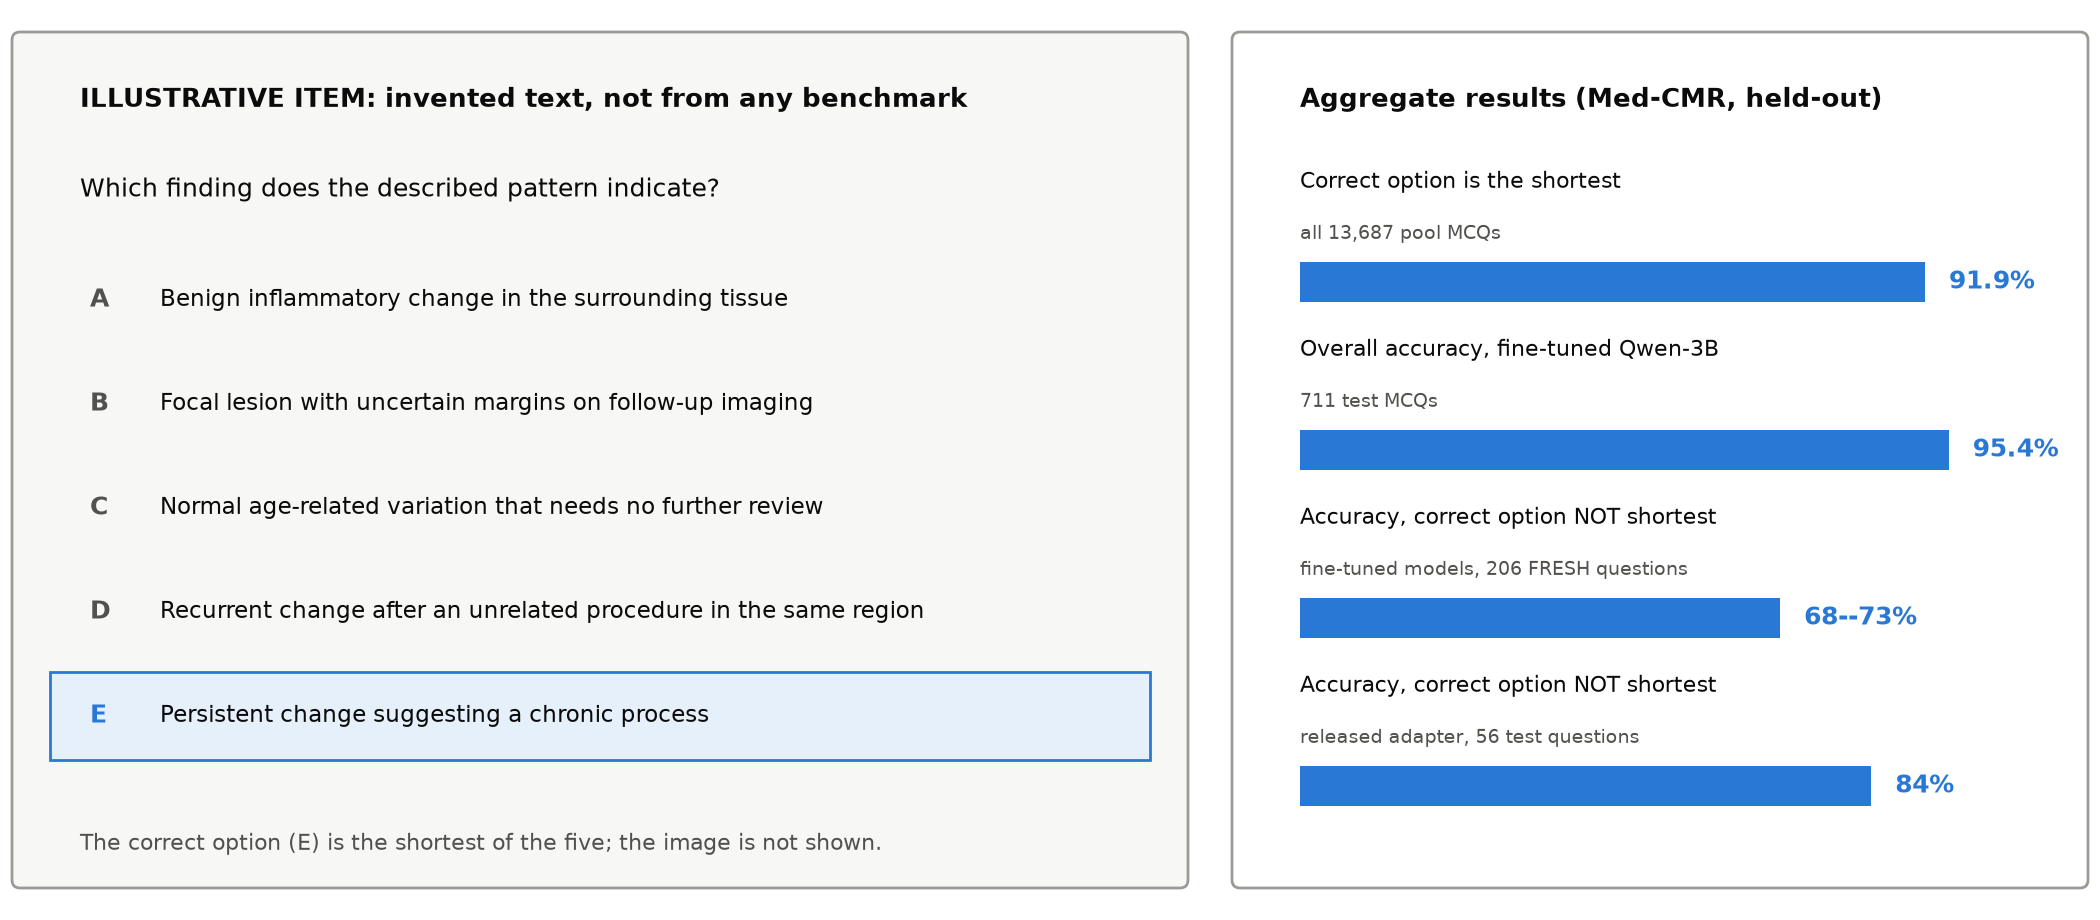
\includegraphics[width=0.76\textwidth]{fig/f1_teaser_illustrative.png}
  \caption{\textbf{An illustrative item and the aggregate numbers it summarises.} The item and its options are invented for illustration and are not from any benchmark; no image is shown. The bars report measured aggregates on Med-CMR: the correct option is the shortest in 91.9\% of the 13{,}687 pool questions; overall accuracy is 95.4\% for fine-tuned Qwen-3B (711 test questions) and 96.1\% for the released adapter; where the correct option is not the shortest, accuracy is 68.0\% and 73.3\% for fine-tuned Qwen-3B and Qwen-7B (206 FRESH questions) and 83.9\% for the released adapter (56 test questions). The bar lengths are schematic.}
  \label{fig:teaser}
\end{figure*}

Studies of medical imaging models have repeatedly reported accuracy that did not rest on disease: COVID-19 chest X-ray models relied on confounding factors and failed in new hospitals~\cite{degrave2021shortcuts}; a pneumonia model performed worse at outside hospitals and could identify a radiograph's source hospital in over 99.9\% of cases~\cite{zech2018variable}; the specificity of a deep learning melanoma classifier fell from 84.1\% to 45.8\% on lesions with surgical skin markings~\cite{winkler2019markings}; and a deployed retinopathy screener met image-quality demands that clinics could not always satisfy~\cite{beede2020humancentered}.
A 2026 preprint reports that frontier models describe images that were never provided and that a text-only model ranked first on a chest X-ray question-answering benchmark~\cite{asadi2026mirage}.
Training on benchmark data can raise scores without the ability~\cite{zhou2023cheater,zhang2024gsm1k}; Figure~\ref{fig:teaser} illustrates the pattern with an invented item; the numbers it summarises are measured on the benchmark, where the training split is the source of the shortcut.
Do vision-language models look at the image?
Audits of medical VQA say mostly not: tuned models lose few points when the image is blanked or swapped~\cite{zafar2026coral}, models ``derive more useful information from the question text than from the image''~\cite{pokrywka2026polish}, and the answer options alone carry exploitable cues~\cite{wang2026medqamm}.
These findings are usually summarised by one number, the average accuracy drop without the image, and read as ``the model ignores the image''.
That number answers the wrong question.
The question that matters is when nonvisual evidence becomes so predictive that additional visual evidence stops helping, and what that leaves for vision to earn.
We call the credit that vision can still earn the benchmark's \emph{visual headroom}: the accuracy of a model with the true image above what it reaches without the image or from option text alone (the \emph{blind ceiling}).
We separate four things that are easily conflated: whether visual information is available (the image is given); whether predictions depend on it (counterfactual images change the answer); whether predictions are accurate because of it (the image adds accuracy above the blind ceiling, which is headroom); and whether the model reasons about the relevant visual content (the right image and region). We test the second throughout and the third through headroom; the fourth is tested only in part (wrong-image identity, blur, occlusion), and we make no claim of semantic understanding.

We answer in six steps, one per section, each about headroom: \textbf{Failure} (Sec.~\ref{sec:obs}): accurate Med-CMR systems have none, on a benchmark whose correct option is the shortest in 91.9\% of the questions; \textbf{Isolation} (Sec.~\ref{sec:setting}): the blind ceiling, counterfactual images, a ladder of image strength and planted shortcuts; \textbf{Quantification} (Sec.~\ref{sec:dose}): planting a shortcut dials headroom from $+13.5$ to $+0.1$ points, at a strength that depends on the benchmark; \textbf{Explanation} (Sec.~\ref{sec:explain}): the cue is sufficient but not the only consumer (option wording and prior knowledge are others); \textbf{Intervention} (Sec.~\ref{sec:remedy}): headroom can be partly bought back for about 4 to 6 points of accuracy, and the bought-back dependence is partly coarse; \textbf{Stress test} (Sec.~\ref{sec:general}): a held-out prediction, the failures and an audit of the challenge's faithfulness judge.
Sec.~\ref{sec:setting} is the method and Secs.~\ref{sec:dose}--\ref{sec:general} are the experiments.

\paragraph{Contributions.}
(i)~A controlled two-axis characterization of the competition between shortcut and visual evidence: image benefit against shortcut strength and image strength (a phase diagram) in a medical and a natural-image benchmark, with a benchmark-dependent lock-out strength ($0.85$ against $0.99$ for Qwen-3B; the first from a grid fixed in advance, the second from a grid extended after a failed prediction, Sec.~\ref{sec:dose}) reported as a measured finding, not a law.
(ii)~What held and what did not: a prediction fixed before the runs held for two further models; three attempts to explain the boundary across benchmarks failed (the benefit without a cue, a one-constant evidence-competition hypothesis, natural variation in text predictability).
(iii)~The visual headroom of four benchmarks (blind ceiling, counterfactual images, a strength ladder): Med-CMR ($-0.1$ points) and OmniMedVQA ($+4.9$) leave almost none, PMC-VQA $+13.7$ and A-OKVQA $+33.2$; average measures rank systems inconsistently.
(iv)~What consumes headroom on Med-CMR and what buying it back costs: the length cue (installed by training on about 1{,}000 questions of the benchmark's own split), wording that resembles the distractors, 96\% overall but 68--73\% (our models) and 84\% (the released system) where length misleads (ids released); about 4 to 6 points of accuracy at 3B and 7B, after ten earlier attempts that did not meet their criteria (Supp.~X), and 11 to 18 points against a plausible wrong image; faithfulness judges that penalise a missing image only when the trace says so.
All tests follow dated, hash-chained amendments (A0--A44), post-hoc criteria are marked and failures are reported.
